\chapter{Volatility: ARCH and GARCH}
\label{cap:garch}

\section{The problem}
Financial returns have three stable features: (i) almost no autocorrelation, (ii) strongly autocorrelated \emph{squares} of returns (volatility comes in waves: calm, turbulence), (iii) heavier tails than a normal. A classic ARMA assumes constant variance and captures none of this.

\section{ARCH(1) and GARCH(1,1)}
Write the (already demeaned) return as $r_t=\sigma_t z_t$, with $z_t$ i.i.d.\ with mean 0 and variance 1. In the \textbf{GARCH(1,1)}:
\[
\sigma_t^2=\omega+\alpha\,r_{t-1}^2+\beta\,\sigma_{t-1}^2,\qquad \omega>0,\ \alpha,\beta\ge0.
\]
\begin{itemize}[leftmargin=1.4em]
\item ARCH(1) is the case $\beta=0$: today's volatility depends only on yesterday's shock.
\item \textbf{Stationarity}: $\alpha+\beta<1$. Unconditional variance: $\omega/(1-\alpha-\beta)$.
\item $\alpha+\beta$ measures \textbf{persistence}. Values close to 1 (such as 0.97) are typical in real data.
\item The kurtosis (of $r_t$) is greater than 3 even with normal $z_t$.
\end{itemize}

\begin{simulacao}[Checked by simulation]
With $\omega=0.1$, $\alpha=0.1$, $\beta=0.85$ and a long simulation (400 thousand points): variance $2.009$ (theory: $0.1/0.05=2$); kurtosis $3.774$ (theory: $3.774$); autocorrelation of $r_t^2$ at lag 1: $0.177$ (theory: $0.179$). The autocorrelation of $r_t$ was close to zero ($0.04$ in a sample of 2000 points), but that of $r_t^2$ was $0.15$. White noise in the returns, strong dependence in the volatility.
\end{simulacao}

\begin{center}
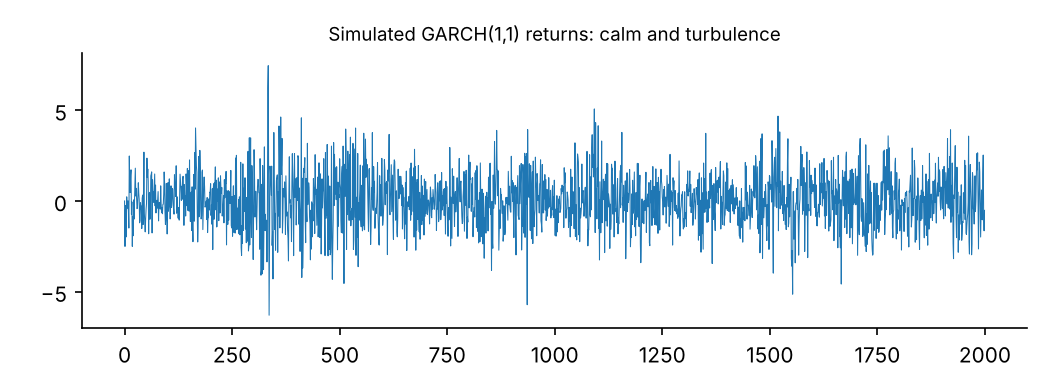
\includegraphics[width=0.9\textwidth]{fig/garch.png}
\end{center}

\begin{simulacao}[Estimation: individual parameters are hard]
Fitting a GARCH(1,1) to 2000 simulated points, I obtained $\hat\omega=0.054$, $\hat\alpha=0.086$ and $\hat\beta=0.890$, against the true $0.1$; $0.1$; $0.85$. The individual parameters missed by quite a bit, but the combination that matters came out close: estimated persistence $0.976$ (true $0.95$) and unconditional variance $0.054/0.024\approx2.26$ (true $2.0$). In very persistent models, $\omega$, $\alpha$ and $\beta$ become strongly correlated in estimation.
\end{simulacao}

\begin{atencao}
\begin{itemize}[leftmargin=1.2em]
\item \textbf{Do not apply ARCH to a series with a unit root or trend}; work with returns (differences of logarithms).
\item \textbf{Symmetric GARCH does not distinguish good news from bad.} For the leverage effect (drops raise volatility more than rises), use GJR-GARCH or EGARCH.
\item \textbf{Choosing normal $z_t$ understates tails}; many use Student's $t$.
\end{itemize}
\end{atencao}

\begin{exercicio}
GARCH(1,1) with $\omega=0.2$, $\alpha=0.1$, $\beta=0.8$. Compute the unconditional variance and the forecast of $\sigma^2_{t+1}$ given $r_t^2=4$ and $\sigma_t^2=3$.
\end{exercicio}
\sol{Unconditional variance: $0.2/(1-0.9)=2$. Forecast: $\sigma^2_{t+1}=0.2+0.1\times4+0.8\times3=0.2+0.4+2.4=3.0$.}

\begin{exercicio}
Why does $\alpha+\beta=1$ create problems, and what is this case called?
\end{exercicio}
\sol{With $\alpha+\beta=1$ the unconditional variance does not exist (the denominator is zero) and volatility shocks never dissipate. This is the IGARCH. The forecast of future volatility no longer reverts to a long-run mean.}
